\documentclass[final]{article}

% if you need to pass options to natbib, use, e.g.:
% \PassOptionsToPackage{numbers, compress}{natbib}
% before loading nips_2017
%
% to avoid loading the natbib package, add option nonatbib:
% \usepackage[nonatbib]{nips_2017}

\PassOptionsToPackage{compress,authoryear,round}{natbib}
\usepackage{nips_2017}

% to compile a camera-ready version, add the [final] option, e.g.:
% \usepackage[final]{nips_2017}

\usepackage[utf8]{inputenc} % allow utf-8 input
\usepackage[T1]{fontenc}    % use 8-bit T1 fonts
\usepackage{hyperref}       % hyperlinks
\hypersetup{colorlinks=true,linkcolor=black,citecolor=black,filecolor=black,urlcolor=black,
            plainpages=false,pdfpagelabels,breaklinks=true,
  pdftitle    = {Brain Tumor Segmentation with Random Forest and U-Net},
  pdfsubject  = {},
  pdfauthor   = {Shuhan Xiao and Alexander Kugele},
  pdfkeywords = {} ,
  pdfcreator  = {pdflatex},
  pdfproducer = {}
}
\usepackage{url}            % simple URL typesetting
\usepackage{booktabs}       % professional-quality tables
\usepackage{amsfonts}       % blackboard math symbols
\usepackage{nicefrac}       % compact symbols for 1/2, etc.
\usepackage{microtype}      % microtypography

\makeatletter
\providecommand*{\input@path}{}
\g@addto@macro\input@path{{fig/}{../figures/}}
\makeatother

\usepackage{graphicx}
\graphicspath{{fig/}{../figures/}}

\usepackage{siunitx}
\usepackage{enumitem}
\usepackage{cleveref}
\usepackage{tikz}
\usetikzlibrary{positioning}

\newcommand*\circled[1]{\tikz[baseline=(char.base)]{%
            \node[shape=circle,fill=blue!0,draw,inner sep=2pt] (char) {#1};}}

\title{Brain Tumor Segmentation with Random Forest and U-Net}

\author{
  Shuhan Xiao \\
  Heidelberg University \\
  \href{mailto:shuhan.xiao@stud.uni-heidelberg.de}{shuhan.xiao@stud.uni-heidelberg.de}\\
  \And
  Alexander Kugele \\
  Heidelberg University \\
  \href{mailto:a.kugele@stud.uni-heidelberg.de}{a.kugele@stud.uni-heidelberg.de}\\
}

\begin{document}

\maketitle

\begin{abstract}
This report compares two methods to segment 2D brain tumor data: A random
forest and a U-Net. It is found that without manual tuning, both methods are
comparable in their segmentation accuracy, achieving Dice scores of $65.9 \%$
and $69.3 \%$ respectively. However, training and inference time of the U-Net
are significantly smaller and training larger datasets is possible more easily.
\end{abstract}

\section{The Dataset}

\subsection{General Information}
Image segmentation is primarily done in two ways: Either designing an algorithm
from first principles or using available data to train an algorithm. As for
this challenge, designing an algorithm without data is very difficult, the
method of choice is training an algorithm from data. For the Multimodal Brain
Tumor Image Segmentation Benchmark \citep{BRATS} in 2015, 3D MR tumor scans
where collected from the BRATS 2012 and BRATS 2013 challenge and from the NIH
Cancer Imaging Archive (TCIA). In total, data for 55 low-grade glioma patients
and 220 high-grade glioma patients is provided. The data is a 16-bit 3D scan of
shape (depth=155, height=240, width=240), where all datasets have been aligned
to the same anatomical template and interpolated to \SI{1}{\mm^3} voxel
resolution. For each patient, four scan types are available: T1, T1c, T2 and
Flair. In the case of the BRATS data, the labels are from expert annotations of
one to four raters. The TCIA data labels were obtained by fusing the results of
multiple segmentation algorithms from the BRATS 2012 and BRATS 2013 challenge
and reviewed by expert raters.\\
Four classes are predefined:
\begin{enumerate}[label=\arabic*),topsep=0pt]
  \setcounter{enumi}{-1}
\item background
\item necrosis
\item edema
\item non-enhancing tumor
\item enhancing tumor
\end{enumerate}
Each 3D image for each scan type is saved in a seperate \verb+.mha+ file. The
average size per file is about \SI{2.2}{MB}, leading to approximately
$\SI{2.2}{MB}\cdot 275 \cdot 4 = \SI{2420}{MB}$ of compressed data.
Uncompressed, the data size increases to over \SI{100}{GB}. In
\cref{fig:dataex}, examples for LGG and HGG and the different scan types are
shown.

\begin{figure}
\centering
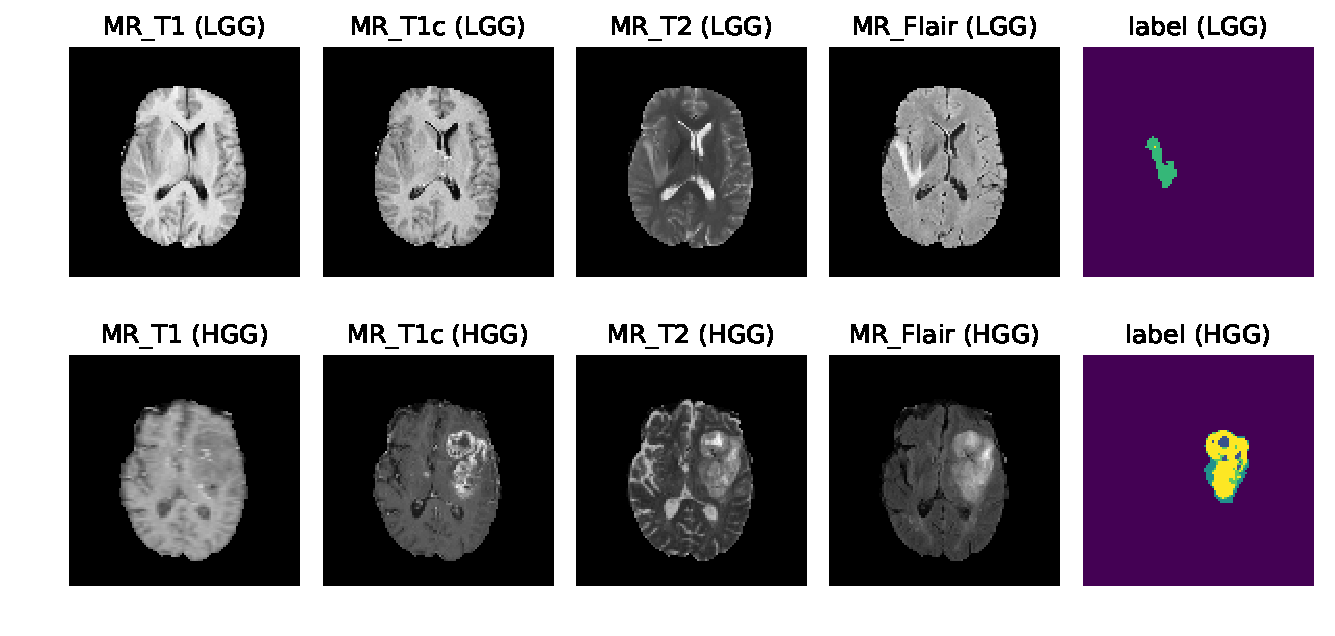
\includegraphics[width=0.99\linewidth]{scan_types_both}
\caption{Dataset examples. \textit{Top:} Low-grade glioma tumor. The structure
is primarily visible in the Flair scan. \textit{Bottom:} High-grade glioma
tumor. The structure is richer and the different scan types help in
differentiating the different types of tumor.}
\label{fig:dataex}
\end{figure}

\subsection{Utilizing the Dataset}
The given images are sliced 3D scans. As we want to do segmentation in two
dimensions, we just take each slice as a separate input image. In total, this
are $155\cdot275\cdot4 = 170500$ input images. This full dataset proved too be
to large to use it for training. After trying out multiple subsets, it was
decided to use only the LGG part of the dataset and to sort out images where
the tumor to background ratio is less than $0.1\%$. This dataset only takes
\SI{110}{MB} compressed on disk. We split this dataset of 3315 images further
up into a training set of 2652 images ($80\%$) and a test set of 663 images.
This dataset is used for both the random forest and the U-Net. The classes are
reduced from five to two: background and tumor. Loading 10 images in the memory
of the GPU for training takes about \SI{3}{GB}. For the random forest, using
1000 images at once takes about \SI{30}{GB} of RAM.

\section{Random Forest}
The random forest is a set of decision trees, where each tree is fitted to a
random subset of the data and predictions are made by taking averages over the
predictions of individual trees. More precisely, given $N$ data points, $N$
points are sampled at random with replacement from the data. These are then
used to train a decision tree. This kind of sampling is called bagging. The
samples that are not used for the training of a decision trees are so-called
out-of-bag samples. These can be used to test the generalization accuracy of
the training.\\
Training of each decision tree in scikit-learn is done with the Classification
and Regression Tree (CART) algorithm.  Before explaining the training
algorithm, the Gini impurity is explained. This measure is used to determine
the next split in a tree. Generally, it can be calculated as
\begin{equation}
G_i = 1 - \sum_{k=1}^{n}p_{i,k}^2
\end{equation}
where $i$ is the node index, $k$ is the class label and $p_{i,k}$ is the ratio
of class $k$ to all classes in the node. The CART algorithm uses a loss based
on this measure
\begin{equation}
J(k, t_k) = \frac{m_L}{m}G_L + \frac{m_R}{m}G_R
\end{equation}
such that it finds for each current leaf a class and a threshold such that the
impurity is minimized for the left and the right leaf to be added. This is done
until the impurity cannot be further reduced or the maximum depth is reached.
The default parameter in scikit-learn is \verb+max_depth=None+, meaning it goes
as deep as it can. This can lead to large trees. An example of one tree after
training is shown in \cref{sec:treevis}, where each small orange or blue dot is
a single node.

\subsection{Features}
A random forest classifies each pixel separately. Therefore, using only the
pixel intensities would only give a good classification if the tumor can be
identified on a single-pixel level. To include information about the local
structure, multiple features are defined, such that each input pixel is an
N-dimensional vector.\\ The features we chose for this task are:
\begin{enumerate}
\item Gaussian filter
\begin{itemize}
\item Convolution with a Gaussian kernel
\item Smoothes the image
\end{itemize}
\item Laplacian of Gaussian (LoG) filter
\begin{itemize}
\item Convolution with the Laplacian of a Gaussian kernel
\item highlights edges (edges are 0)
\end{itemize}
\item Gaussian gradient magnitude filter
\begin{itemize}
\item Convolution with the gradient of a Gaussian kernel
\item highlights edges (edges are extrema)
\end{itemize}
\item Eigenvalues of the Hessian matrix
\begin{itemize}
\item determines the surface concavity
\end{itemize}
\item Eigenvalues of the structure tensor
\begin{itemize}
\item Summarizes gradient direction
\end{itemize}
\item Equalized histogram
\begin{itemize}
\item Enhances contrast
\end{itemize}
\end{enumerate}

Except for the equalized histogram, they all share the tuneable kernel width
$\sigma$, which is set to $\{0.3, 0.7, 1., 3.5\}$. In total, $N=29$ filters are
used. In \cref{fig:features}, the features are shown for one example image of
the dataset for $\sigma = 0.3$. The tumor region in the bottom left can be
clearly identified for the Gaussian (bright), Laplacian of Gaussian (dark) and
the equalized histogram (bright). However, for other examples the tumor is also
pronounced in the other features.

In principle one could also utilize the different scan types as features.
However, the dataset is already very big and therefore it was decided to not
take the other scan types as features. This also allows for a fair comparison
between the random forest and the U-Net, as they are then trained with the same
dataset.\\

\begin{figure}
\centering
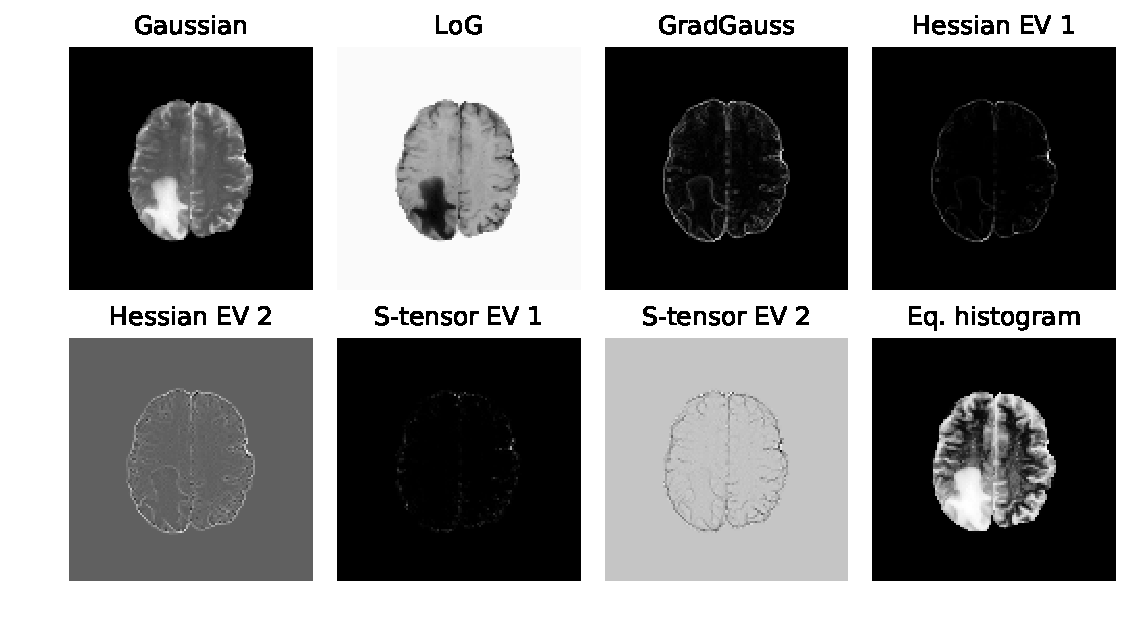
\includegraphics[width=0.99\textwidth]{features}
\caption{Features for the random forest. The Gaussian, Laplacian of Gaussian
and the equalized histogram enhance the tumor region. In this example, the
eigenvalues of the structure tensor and the Hessian matrix are not significant
for the classification. However, they improved the classification on a small
test set and therefore are also kept.}
\label{fig:features}
\end{figure}

\subsection{Batch-mode training}
Using the features defined in the last section, the complete training data
still takes about \SI{70}{GB} of memory. Therefore, it is decided to train the
random forest sequentially on large chunks of the dataset as suggested in
\cite{batchrf}. The dataset is divided in three batches of about \SI{26}{GB}
each, assuming that in each large batch, the distribution of features is
approximately equal. Then, we train a random forest on 100 estimators for each
batch. The resulting random forest therefore has 300 estimators. It takes
approximately \SI{15}{GB} on disk, saved in the pickle format. In scikit-learn,
the \verb+warm_start=True+ parameter of the Random Forest can be used to do
this kind of batch-mode training.

\section{RF: Results}
Training the random forest took about \SI{13}{h}. Storing it on disk takes
about \SI{15}{GB} in pickled format. Both training time and classifier disk
size can be reduced by setting adjusting the hyperparameters \verb+max_depth+,
\verb+min_impurity_leaf+, \verb+max_leaf_nodes+, \verb+min_samples_split+,
\verb+min_samples_leaf+. However, finding a good setup is also time-consuming
and we mainly want to compare the segmentation accuracy. Therefore, the
standard values are kept. Therefore, loading the classifier takes about
\SI{310}{s} and a single prediction takes about \si{2-20}{s}. In
\cref{fig:rfresults}, an example for the segmentation of test image 84 is shown
together with the box plots for the Dice score, sensitivity and specificity.
The mean scores are Dice$=65.9 \%$, sensitivity$=\num{77.1} \%$ and
specificity$=\num{99.1} \%$.

\begin{figure}
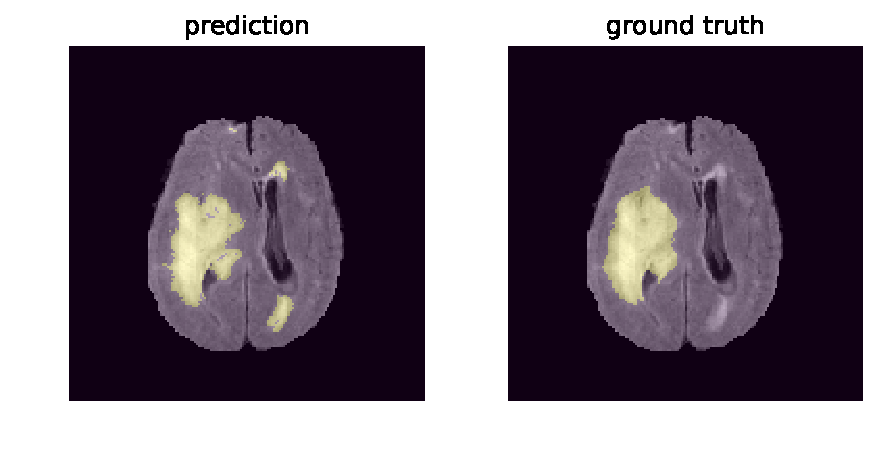
\includegraphics[width=0.49\textwidth]{rf_prediction_84}
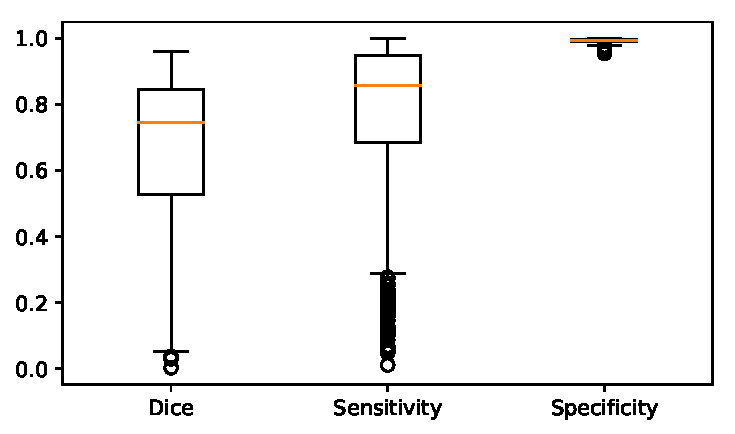
\includegraphics[width=0.49\textwidth]{boxplot_rf}
\caption{\textit{Left:} Example for a prediction on image 84 of the test set.
The true tumor is segmented very precisely, but other smaller bright areas are
also incorrectly classified as being a tumor. \textit{Right:} Boxplots for the
Dice score, sensitivity and specificity. As most of the images are background,
the specificity is very high and has a low standard deviation. The quantiles
$Q_1$ (25th percentile) to $Q_3$ (75th percentile) span almost over the whole
range of the Dice score and sensitivity. This means that for a single image,
the classification can vary significantly.}
\label{fig:rfresults}
\end{figure}

\section{Conclusion}
Both techniques lead to similar segmentation accuracies. Training and inference
time with the U-Net are significantly smaller and it is expected to be able to
increase the segmentation accuracy by a deeper U-Net, longer training time,
more training data and hyperparameter tuning. To increase the prediction
accuracy of the random forest, new features have to be introduced. As it is
difficult to decide which features will lead to better results, improving the
U-Net is easier. Also, adding more training data does only lead to a longer
training time for the U-Net, but for the random forest it additionally requires
more memory resources, making this method less flexible.

\section{Appendix}

\subsection{Hardware Specifications}
This section lists the hardware details of the machine used to train the random
forest and the U-Net. This makes the given times more comparable to other
systems.
\begin{itemize}
\item Intel Core i5-3550 CPU \@ 3.30GHz
\item Nvidia Geforce GTX 1060 6GB
\item 8 GB RAM
\item 40 GB swap on SSD
\end{itemize}

\clearpage
\subsection{Visualization of a single tree}
\label{sec:treevis}
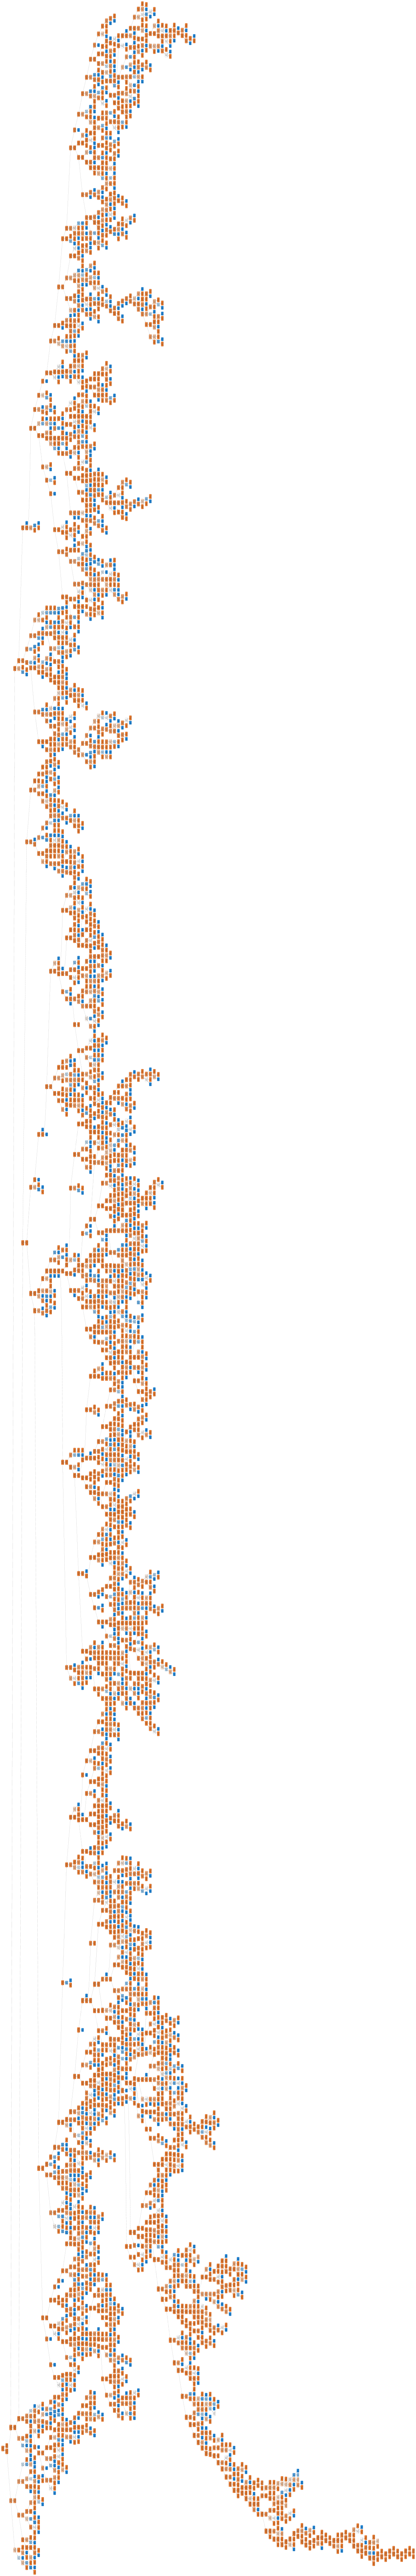
\includegraphics[width=0.94\textwidth,height=0.94\textheight]{Tree4.png}

\bibliographystyle{plainnat}
\bibliography{../biblio}\vspace{0.75in}

\end{document}
